\subsection{Inteligencia artificial en el reciclaje}

\textbf{Otra tecnología emergente con la que se está experimentando en el campo del reciclaje es la utilización de inteligencia artificial o IA.} Los algoritmos de la IA pueden analizar grandes cantidades de datos y aprender de ellos para mejorar la eficiencia del proceso de reciclaje. Por ejemplo, se pueden utilizar sistemas de aprendizaje automático para identificar materiales específicos en los residuos y separarlos con mayor precisión. 

Además, la IA también podría ayudar a predecir cuánto material se puede reciclar de un lote específico de residuos, lo que permitiría una mejor planificación y gestión del proceso de reciclaje. Aunque esta tecnología todavía está en una etapa temprana de implementación~\cite{ecoembes}.

\subsection{Sostenibilidad}

Cada vez más, la tecnología cobra un papel más importante a la hora de dar respuesta a los desafíos a nivel medioambiental, social y económico a los que nos enfrentamos actualmente. Los avances tecnológicos han permitido avanzar hacia un desarrollo global sostenible.

Las tecnologías sostenibles se conocen como aquellas que están enfocadas en los principios de sostenibilidad. Son aquellas que a través de la reutilización, el reciclaje, la conservación de recursos naturales y de la eficiencia energética, reducen la contaminación. Por lo tanto, minimizan el impacto ambiental.

Ciertamente, las tecnologías sostenibles tienen muy presentes las diferentes necesidades de la sociedad. Además, estas tecnologías implicadas con el desarrollo sostenible, emplean menos energía para realizar los procesos, emplean una cantidad menor de recursos limitados. Por consecuencia, reducen la utilización de los recursos naturales en todas sus etapas (creación, puesta en marcha o utilización)~\cite{caputo}.

\subsection{Microcontroladores} 

Un microcontrolador es un circuito integrado de alta escala de integración que incorpora la mayor parte de los elementos que configuran un controlador. Un microcontrolador dispone normalmente de los siguientes componentes:
\begin{itemize}
    \item Procesador o UCP (Unidad Central de Proceso).
    \item Memoria RAM para contener los datos.
    \item Memoria para el programa tipo ROM/PROM/EPROM.
    \item Líneas de E/S para comunicarse con el exterior.
    \item Diversos módulos para el control de periféricos (temporizadores, Puertas Serie y Paralelo, CAD: Conversores Analógico/Digital, CDA: Conversores Digital/Analógico, etc.).
    \item Generador de impulsos de reloj que sincronizan el funcionamiento de todo el sistema.
\end{itemize}

El microcontrolador es, en definitiva, un circuito integrado que incluye todos los componentes de un computador. Debido a su reducido tamaño es posible montar el controlador en el propio dispositivo al que gobierna. En este caso, el controlador recibe el nombre de controlador empotrado (embedded controller)~\cite{microcontroladores}.

El microcontrolador nace cuando las técnicas de integración han progresado lo bastante para permitir su fabricación; pero también porque, muy a menudo, tanto en las aplicaciones domésticas como industriales, se tiene la necesidad de sistemas “inteligentes” o, al menos, programables. Un ejemplo muy simple es el programador de una lavadora, el cual debe controlar una cierta cantidad de elementos con ciclos y cadencias perfectamente definidas, pero variables en función del programa seleccionado. Otras aplicaciones más técnicas tienen, igualmente, necesidad de sistemas programables. Por ejemplo, una fotocopiadora debe controlar permanentemente un gran número de elementos y de funciones. Gracias a la llegada de los microcontroladores, tarjetas que contenían varias decenas de circuitos lógicos clásicos se han visto reducidas a dos o tres microcontroladores.

\begin{figure}[H]
    \centering
    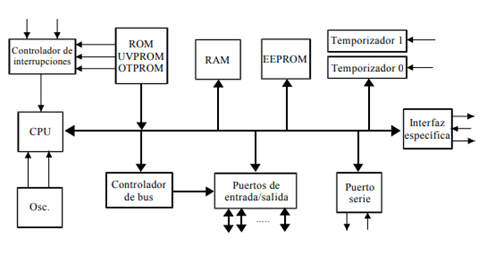
\includegraphics[scale = 0.95]{Imagenes/CAP2_elementos_microcontrolador.png}
    \caption{Elementos de un microcontrolador}{Fuente: Adaptado de~\cite{microcontroladores}}
\end{figure}
